\subsection{Stable slices of the twelve marked families}
\label{sec:stable-zipper-slices}

For each plane-orientation choice $\kappa$ and endpoint signature $e$, let
\[
 \mathcal S_{\kappa,e}
 =\{q\in\Omega:F_{1,q}K_q\cap F_{2,q}K_q=\{q\}\}.
\]
This is the stable set of that marked zipper surface. The parameters in
$\Omega\setminus\mathcal S_{\kappa,e}$ still give connected attractors;
their canonical curves have additional identifications. In particular,
these plots resolve structure \emph{within} the connectedness loci.
The signs of $\kappa$ describe orientation in the plane, while the bits of
$e$ describe traversal of the two curve pieces.

\begin{proposition}[A common necessary disk]
\label{prop:zipper-necessary-disk}
For every marked binary planar zipper,
\[
 (0,1)\subset\mathcal S_{\kappa,e}
 \subset \mathbb D_{1/2}:=\{q:|q-\tfrac12|<\tfrac12\}.
\]
\end{proposition}
\begin{proof}
The real interval was established above. If the canonical curve is
embedded, its two pieces meet in one point. The planar finite-intersection
theorem of Bandt and Rao~\cite{BandtRao2007} therefore gives the open set
condition. Choose a bounded nonempty feasible open set $O$ (intersect a feasible open
set with a sufficiently large forward-invariant open ball) and write
$r_1=|q|$, $r_2=|1-q|$. The disjoint sets $F_1(O),F_2(O)\subset O$ imply
$r_1^2+r_2^2\le1$ by planar area. Equality is impossible for a Jordan arc:
in that case $O\setminus\bigcup_{|u|=n}F_u(O)$ has area zero for every $n$,
so the latter union is dense in $O$. Its distance from $K$ tends uniformly
to zero as $n\to\infty$, which implies $O\subset K$. An arc has empty
interior. Hence $|q|^2+|1-q|^2<1$, equivalent to the displayed disk.
\end{proof}

In the atlas coordinates this necessary disk is
$\rho>2\sqrt{w^2+(1-w)^2}$. Stable zipper parameters therefore lie between
the guaranteed connected core and the outer bound $\rho\le2$; the real
interval occupies $\rho=2$.

\begin{proposition}[An exact reversing zipper slice]
\label{prop:oo00-stable-disk}
For $\kappa=(-,-)$ and $e=(0,0)$, the stable set is exactly
$\mathcal S_{--,00}=\mathbb D_{1/2}$. If $q\notin\mathbb R$ lies on its
boundary circle, the attractor is the filled triangle
$T_q=\operatorname{conv}\{0,q,1\}$ and the two pieces meet in the segment
$[q,|q|^2]$.
\end{proposition}
\begin{proof}
Conjugation permits $\Im q>0$. Put $x=\Re q$ and $s=|q|^2$. The maps are
$F_1(z)=q\overline z$ and $F_2(z)=q+(1-q)\overline z$, and their triangle
images are
\[
 F_1(T_q)=\operatorname{conv}\{0,q,s\},\qquad
 F_2(T_q)=\operatorname{conv}\{q,1,2x-s\}.
\]
The strict contraction lens ensures $0<s<1$ and $0<2x-s<1$, so both images
are contained in $T_q$. When $q\in\mathbb D_{1/2}$, we have $s<x$;
the base intervals $[0,s]$ and $[2x-s,1]$ are disjoint and the triangles
meet only at $q$. Thus $K_q\subset T_q$ and its first-level pieces meet
only at $q$, proving embeddedness. For real $q\in(0,1)$ the attractor is
the interval and embeddedness follows directly. The necessary-disk
proposition excludes every remaining parameter. On the nonreal circle
$s=x$, the two triangles exactly tile $T_q$ and share the segment from
$q$ to $s$; uniqueness of the attractor gives the asserted filled triangle.
\end{proof}

\subsection{Two further exact stable disks}
\label{subsec:oo01-oo10-exact-disk}

The opposite--opposite endpoint signatures $01$ and $10$ have the
same complete stable disk as signature $00$. In particular, these
families supply exact cases with no stable islands.

\begin{theorem}[Exact stable disks for the reversing signatures $01$ and $10$]
\label{thm:oo01-oo10-stable-disks}
For the opposite--opposite binary zippers with endpoint signatures
$e=(0,1)$ and $e=(1,0)$,
\[
 \mathcal S_{--,01}=\mathcal S_{--,10}
 =\left\{q:\left|q-\frac12\right|<\frac12\right\}.
\]
Put $s=|q|^2$ and $t=|1-q|^2$. In the $01$ case an invariant
triangle on the stable disk is
\[
 T_{01}(q)=\operatorname{conv}\left\{0,1,\frac{q}{1-t}\right\};
\]
in the $10$ case it is
\[
 T_{10}(q)=\operatorname{conv}\left\{0,1,\frac{q-s}{1-s}\right\}.
\]
For nonreal $q$ on the boundary circle $s+t=1$, the respective
attractors are these filled triangles. The first-level intersection
is $[q,1]$ for signature $01$, and $[0,q]$ for signature $10$.
\end{theorem}
\begin{proof}
Consider signature $01$, whose maps are
\[
 F_1(z)=q\overline z,\qquad
 F_2(z)=1-(1-q)\overline z.
\]
Complex conjugation permits $\Im q=y>0$. The real interval
$q\in(0,1)$ gives an embedded interval directly. Define
\[
 C=\frac{q}{1-t},\qquad A=\frac{s}{1-t}.
\]
The contraction lens gives $0<t<1$. A direct calculation gives
\[
 F_2^2(z)=q+tz,\qquad F_2(C)=C,
\]
and hence
\begin{align*}
 F_1(T_{01})&=\operatorname{conv}\{0,q,A\},\\
 F_2(T_{01})&=\operatorname{conv}\{1,q,C\}.
\end{align*}
Inside the disk, $s+t<1$, so $0<A<1$ and
$q=(1-t)C$ lies strictly between $0$ and $C$. Every displayed vertex
therefore lies in $T_{01}$, proving invariance.

The line through $q$ and $1$ separates these two image triangles.
More explicitly, the real-linear functional
\[
 \ell(z)=\Im\bigl(\overline{(1-q)}(z-q)\bigr)
\]
obeys
\[
 \ell(0)=-y<0,\quad
 \ell(A)=(A-1)y<0,\quad
 \ell(q)=\ell(1)=0,\quad
 \ell(C)=\frac{t}{1-t}y>0.
\]
Thus $F_1(T_{01})$ meets the separating line only at $q$, while
$F_2(T_{01})$ lies on the other closed side. Their intersection is
exactly $\{q\}$. The attractor lies in $T_{01}$, so its first-level
pieces also meet exactly at their prescribed join. The binary
embedding criterion proves embeddedness throughout the disk.
The common necessary-disk theorem excludes every remaining parameter
in the contraction lens.

On the nonreal boundary $s+t=1$, one has $A=1$. The two image
triangles then partition $T_{01}$ along $[q,1]$ because $q$ lies on
the side $[0,C]$. Consequently their union is $T_{01}$, and uniqueness
of the attractor gives the asserted filled triangle and overlap.

Finally, endpoint reflection $z\mapsto1-z$ with generator exchange
sends signature $01$ at $1-q$ to signature $10$ at $q$. It sends
$T_{01}(1-q)$ to
\[
 \operatorname{conv}\left\{0,1,
 1-\frac{1-q}{1-s}\right\}
 =T_{10}(q)
\]
and sends the shared boundary segment $[1-q,1]$ to $[0,q]$.
\end{proof}

The finite return tests below also apply to these signatures, but the
triangle proof already classifies their complete stable sets.


\paragraph{Finite certificates in seven marked slices.}
A common endpoint return turns the prescribed contact into a finite
verification. Word maps are composed from left to right in symbolic order,
so $F_{12}=F_1\circ F_2$. The following table gives seed words $U,V$,
return words $r,s$, and the multiplier $\eta$ of a common similarity
$H(z)=q+\eta(z-q)$ satisfying
\begin{equation}\label{eq:zipper-return-identities}
 F_{Ur}=H\circ F_U,\qquad F_{Vs}=H\circ F_V.
\end{equation}
Every row holds identically on the contraction lens.
\begin{center}
\begin{tabular}{cc|cc|cc|c}
Plane type&$e$&$U$&$V$&$r$&$s$&$\eta$\\\hline
DD&01&12&22&1&1&$q$\\
DD&10&11&21&2&2&$1-q$\\
DD&11&1&2&12&21&$q(1-q)$\\
DO&10&11&21&22&22&$|1-q|^2$\\
DO&11&1&2&1212&2121&$|q|^2|1-q|^2$\\
OO&01&12&22&11&11&$|q|^2$\\
OO&10&11&21&22&22&$|1-q|^2$
\end{tabular}
\end{center}
Here DO means that $F_1$ is direct and $F_2$ opposite. The identities follow
by composition; in the rows with a reversing endpoint return, taking its
square produces the displayed positive real multiplier. Since $|\eta|<1$,
$H$ is a strict contraction fixing the join.

\begin{proposition}[A finite certificate for an embedded zipper]
\label{prop:zipper-return-certificate}
Fix one row of the table, put $d=|U|=|V|$ and $m=|r|=|s|$, and suppose:
\begin{enumerate}
\item among the pairs $F_uK\cap F_vK$ with $|u|=|v|=d$, $u_1=1$,
      $v_1=2$, every pair other than $(U,V)$ is empty;
\item among the pairs $F_{Uu}K\cap F_{Vv}K$ with $|u|=|v|=m$,
      every pair other than $(r,s)$ is empty.
\end{enumerate}
Then $q\in\mathcal S_{\kappa,e}$. Every required empty intersection can
be certified by a finite cover by rigorously disjoint cylinder disks.
Conversely, at every parameter in $\mathcal S_{\kappa,e}$ both conditions
hold and all these disk tests eventually terminate in exact arithmetic.
In particular, the
seven stable slices in the table are open in $\Omega$.
\end{proposition}
\begin{proof}
The first condition gives $F_1K\cap F_2K=J:=F_UK\cap F_VK$.
The second and~\eqref{eq:zipper-return-identities} give $J=H(J)$.
The compact set $J$ contains $q$ and a strict contraction has only one
nonempty compact invariant set, namely its fixed point. Hence $J=\{q\}$.

For the finite test, use the invariant disk $B=\overline D(1/2,R)$, where
\[
 R=\max\left\{\frac{|1-q|}{2(1-|q|)},
                 \frac{|q|}{2(1-|1-q|)}\right\}.
\]
Both maps send its centre to $q/2$ and $(1+q)/2$, respectively, regardless
of plane orientation or endpoint signature; the formula ensures
$F_j(B)\subset B$. Thus $K\subset B$. To establish any required
$F_uK\cap F_vK=\varnothing$, recursively replace that pair by its four
child pairs, discarding a pair whenever its two cylinder disks are
rigorously disjoint. Termination gives a finite cover proving emptiness.
Conversely, every such empty compact intersection has positive distance,
so this particular pair test eventually terminates in exact arithmetic.

For the converse, an embedded curve has unique endpoint addresses, as in
Proposition~\ref{prop:binary-embedding}. The two addresses of its join are
$121^\infty,221^\infty$ for signature 01;
$112^\infty,212^\infty$ for signature 10; and
$1(12)^\infty,2(21)^\infty$ for signature 11. In each row of the table,
$(U,V)$ is their pair of length-$d$ prefixes and $(Ur,Vs)$ the corresponding
pair of length-$d+m$ prefixes. Therefore no other tested pair contains
the join. Since the two first-level pieces meet only there, all those
other pairs are disjoint. The finite tests consequently terminate.
Their strict separation inequalities persist locally, which proves
openness.
\end{proof}

All conditions in a terminating disk test are strict. When evaluated
with outward bounds for a rational rectangle in the $q$-plane, they
certify \emph{every} parameter in that rectangle. A stopped or capped
test is unresolved and is not evidence of an additional contact.
The DD11 row is the join-renormalization mechanism used for
wiggles~\cite{Calegari2026}; the table records the endpoint returns
needed for the other marked presentations.

\paragraph{Symmetries and interpretation.}
Complex conjugation carries each stable slice to itself. Endpoint
reflection $z\mapsto1-z$, with the two generators exchanged, carries
$(\kappa_1,\kappa_2;e_1,e_2;q)$ to
$(\kappa_2,\kappa_1;e_2,e_1;1-q)$. Thus the DD and OO columns 01 and 10
are reflected companions. In the mixed case that operation interchanges
the labels of the direct and opposite maps; it must not be used to
identify the displayed DO columns without retaining the relabelling.


\subsection{Four stable slices in exterior coordinates}
\label{sec:exterior-zipper-atlas}

The comparative figures use DD$(1,0)$, DD$(1,1)$, DO$(1,0)$ and
DO$(1,1)$. The first DD signature represents the reflected pair
$01,10$; retaining one of them makes the four-family comparison more
direct. Each displayed region is a subset of a two-real-dimensional
zipper surface in an ambient four-real-dimensional parameter space.
The following exterior coordinates place these surfaces in a common
geometric display while keeping the fourth coordinate explicit.

For canonical coefficients $(a,b)$, put
\begin{equation}\label{eq:exterior-canonical-coefficients}
 c_1=1/a,\qquad c_2=1/b.
\end{equation}
The strict contraction domain is exactly $|c_1|>1$, $|c_2|>1$.
These are reciprocal coefficients; if a generator is opposite, its
inverse map is $S_j^{-1}(z)=J_{\kappa_j}(c_j(z-t_j))$, with
$t_1=-1,t_2=1$. In particular, the conjugation remains part of the
inverse map.

It is useful to distinguish this canonical pair from the unsigned
endpoint coordinates
\begin{equation}\label{eq:exterior-endpoint-coordinates}
 c=\frac1q,\qquad v=\frac1{1-q}=\frac{c}{c-1},\qquad
 (c-1)(v-1)=1.
\end{equation}
The contraction lens becomes $|c|>1$, $\Re c>1/2$, and the common
necessary condition for stability becomes the half-plane $\Re c>1$.
Thus the reciprocal chart makes the stable-set bound linear. The
planar panels below use this $c$ coordinate. For all four selected
families the canonical first coefficient is instead $c_1=-c$.

\begin{proposition}[Exterior placement of the four selected surfaces]
\label{prop:four-exterior-surfaces}
Write $q=x+iy$, $s=|q|^2$, and set
\[
 N_{10}=3x-2y^2+iy(2x-1),\qquad
 N_{11}=1+q+s(2q-1).
\]
Both quantities are nonzero throughout $\Omega$. For the selected
signatures $e=(1,e_2)$, the canonical exterior coefficients are
\begin{equation}\label{eq:four-exterior-surfaces}
\begin{array}{c|cc}
\text{plane type}&c_1&c_2\\\hline
\mathrm{DD}&-c&(-1)^{e_2}v\\[2pt]
\mathrm{DO}&-c&(-1)^{e_2}v\,N_{1e_2}/\overline{N_{1e_2}}.
\end{array}
\end{equation}
Consequently the DO surfaces include a nonconstant phase rotation of
the opposite coefficient. Their endpoint equations alone do not give
their placement in the canonical coefficient chart.
\end{proposition}
\begin{proof}
Direct coefficients are unchanged by complex-affine conjugacy, giving
the DD row. For DO, the first endpoint map is $F_1(z)=q-qz$ and the
second has coefficient $B=(-1)^{e_2}(1-q)$ multiplying $\overline z$.
Put $D=3(1+2x)$. Solving for the fixed point $m$ of
$(F_1+F_2)/2$ gives
\[
 m_{10}=\frac{4q+2\overline q}{D},\qquad
 m_{11}=\frac{1+3q+2s}{D}.
\]
The normalizing displacement in
Proposition~\ref{prop:canonical-normalization} is
$d=F_2(m)-m=m-F_1(m)=(1+q)m-q=N_{1e_2}/D$.
Hence $a=-q$ and $b=B\overline d/d=B\overline N/N$, proving
the formula after reciprocation. The lens has $0<x<1$, so $D>0$.
If $N_{10}=0$, its imaginary part forces either $y=0$ or $x=1/2$.
In the first case its real part is $3x>0$; in the second it is
$3/2-2y^2>0$ because $y^2<3/4$. Finally,
$\Re N_{11}=1-s+x(1+2s)>0$, since $s<1$ and $x>0$.
\end{proof}

\paragraph{Projection of the four-dimensional atlas.}
Use the canonical coefficient phases
\[
 \theta_1=\arg a=\alpha-\gamma,\qquad
 \theta_2=\arg b=-\alpha-\gamma
 \pmod{2\pi}.
\]
Together with
\begin{equation}\label{eq:exterior-weight-radial}
 w=\frac{|c_2|}{|c_1|+|c_2|},\qquad
 \rho=\frac{2|c_1||c_2|}{|c_1|+|c_2|},
\end{equation}
these give four real coordinates. Define
\begin{equation}\label{eq:zipper-three-dimensional-projection}
\begin{split}
 X&=(4+\rho\cos\theta_1)\cos\theta_2,\\
 Y&=(4+\rho\cos\theta_1)\sin\theta_2,\\
 Z&=\rho\sin\theta_1.
\end{split}
\end{equation}
This map respects the phase lattice~\eqref{eq:phase-lattice}. At any
fixed $w$, it is injective on the connectedness range $0<\rho\le2$:
if $R=\sqrt{X^2+Y^2}$, then
\[
 \rho=\sqrt{(R-4)^2+Z^2},\quad
 \theta_1=\arg(R-4+iZ),\quad
 \theta_2=\arg(X+iY).
\]
Across different weights the display omits one coordinate. Colour
records $w$, so the projected position together with its numerical
weight recovers the exterior pair
\[
 c_1=\frac{\rho}{2w}e^{-i\theta_1},\qquad
 c_2=\frac{\rho}{2(1-w)}e^{-i\theta_2}.
\]
Projected overlaps at distinct weights do not assert intersections
in four dimensions. DD and DO remain separate discrete orientation
classes and are displayed separately.

On every zipper surface,
$w=|q|/(|q|+|1-q|)$ and $\rho=2/(|q|+|1-q|)$. Its stable set lies in
\begin{equation}\label{eq:exterior-stable-band}
 2\sqrt{w^2+(1-w)^2}<\rho\le2.
\end{equation}
The wireframe $\rho=2$ in Figure~\ref{fig:zipper-stable-atlas} is an
outer coordinate reference. It is not a computed connectedness
boundary. The central opening is imposed by the toroidal projection.

\paragraph{Certified stable regions and linked curve probes.}
The coloured surfaces and planar regions are images of closed parameter
cells certified by Proposition~\ref{prop:zipper-return-certificate}.
Their union is a finite inner cover of the stable set. The figures
show this positive evidence without assigning a membership class to
the unpainted part of the plane or the projection. In particular,
an apparent gap between cells is not a proved barrier, and the edge
of the displayed cover need not be a stable-set boundary. Curved
images of cells are drawn by a finite mesh; the underlying
certificate is attached to the original $q$ cell. The exterior panels
show the finite window $0.96\le\Re c\le4.65$,
$-2.70\le\Im c\le0.13$. Their lower half corresponds to
$\Im q\ge0$; conjugation gives the other half. The unbounded
tail as $q\to0$ continues beyond the window.

The same three endpoint parameters link each selected family to
three planar curve examples:
\begin{equation}\label{eq:three-shared-zipper-probes}
 q_A=\tfrac12+\tfrac15i,\qquad
 q_B=\tfrac12+\tfrac25i,\qquad
 q_C=L=\frac{272727+347877i}{800000}.
\end{equation}
The parameters $q_A,q_B$ are certified stable in all four families.
At $q_C$, DD$(1,1)$ and DO$(1,1)$ are certified stable. The DD case
is the point in Calegari's disconnected wiggle locus. At the same
endpoint parameter, DO$(1,0)$ has an additional identification,
certified by the exact degree calculation described in
Appendix~\ref{app:zipper-computation}. The present certificates do
not classify DD$(1,0)$ at $q_C$. The three examples therefore compare
the geometry of the four marked families at common parameters;
they do not assert that all twelve curves are embedded.

\begin{figure}[p]
\centering
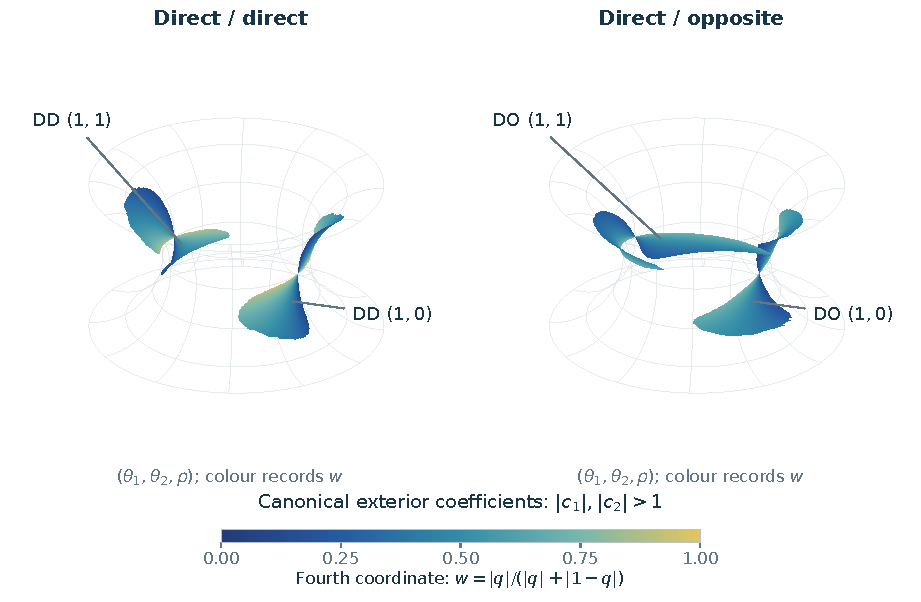
\includegraphics[width=\textwidth]{figures/four_family_projection.pdf}
\caption{Four selected stable slices placed in the four-dimensional
atlas by exterior coefficients $|c_1|,|c_2|>1$ and projected using
\eqref{eq:zipper-three-dimensional-projection}. DD and DO occupy
separate orientation charts. Colour records the fourth coordinate
$w$; the visible sheets consist of certified stable parameter cells.
The wireframe is the outer reference $\rho=2$. Position alone omits
$w$, and the imposed toroidal opening has no implication for the
topology of the connectedness locus. The canonical DO phase rotation
is included as in~\eqref{eq:four-exterior-surfaces}.}
\label{fig:zipper-stable-atlas}
\end{figure}

\begin{figure}[p]
\centering
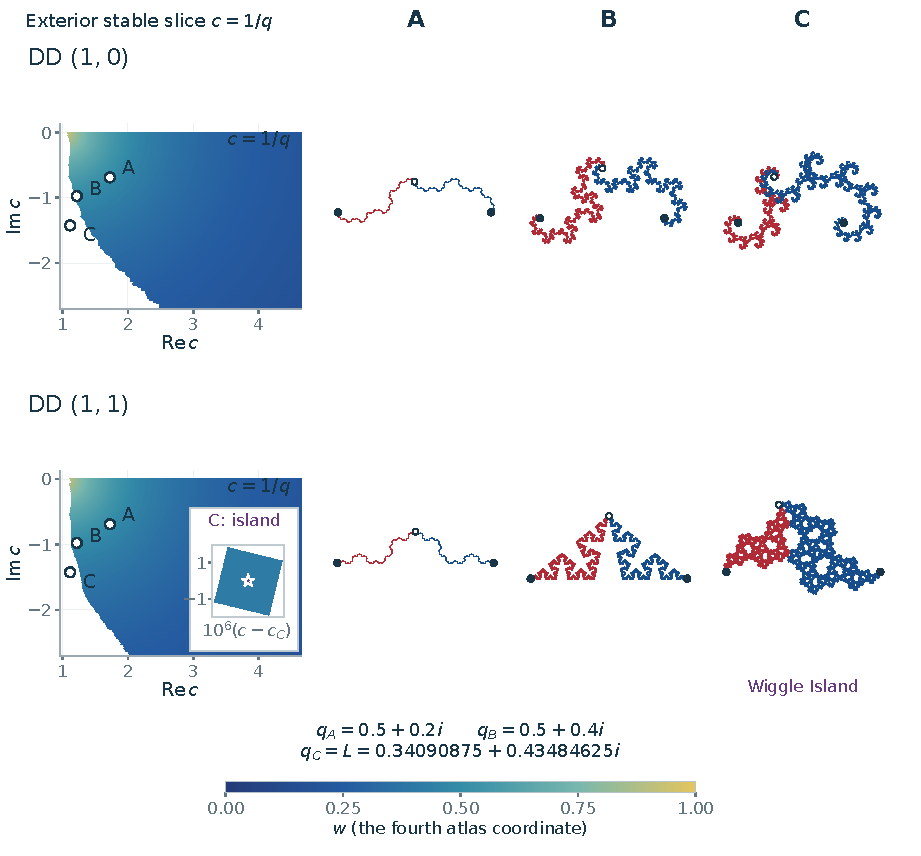
\includegraphics[width=\textwidth]{figures/four_family_DD.pdf}
\caption{DD$(1,0)$ and DD$(1,1)$: certified stable inner covers in the
unsigned endpoint coordinate $c=1/q$, linked to the three common
curve probes~\eqref{eq:three-shared-zipper-probes}. The corresponding
canonical exterior coordinates are $c_1=-c$ and
$c_2=(-1)^{e_2}c/(c-1)$. The DD$(0,1)$ reflection is represented
by DD$(1,0)$. Red and blue distinguish the first-level curve pieces;
they are not membership labels. The tiny certified DD$(1,1)$
neighbourhood of $L$ is shown separately from the common-scale cover.
The curve approximations and their error bounds are recorded in
Appendix~\ref{app:zipper-computation}.}
\label{fig:zipper-dd-gallery}
\end{figure}

\begin{figure}[p]
\centering
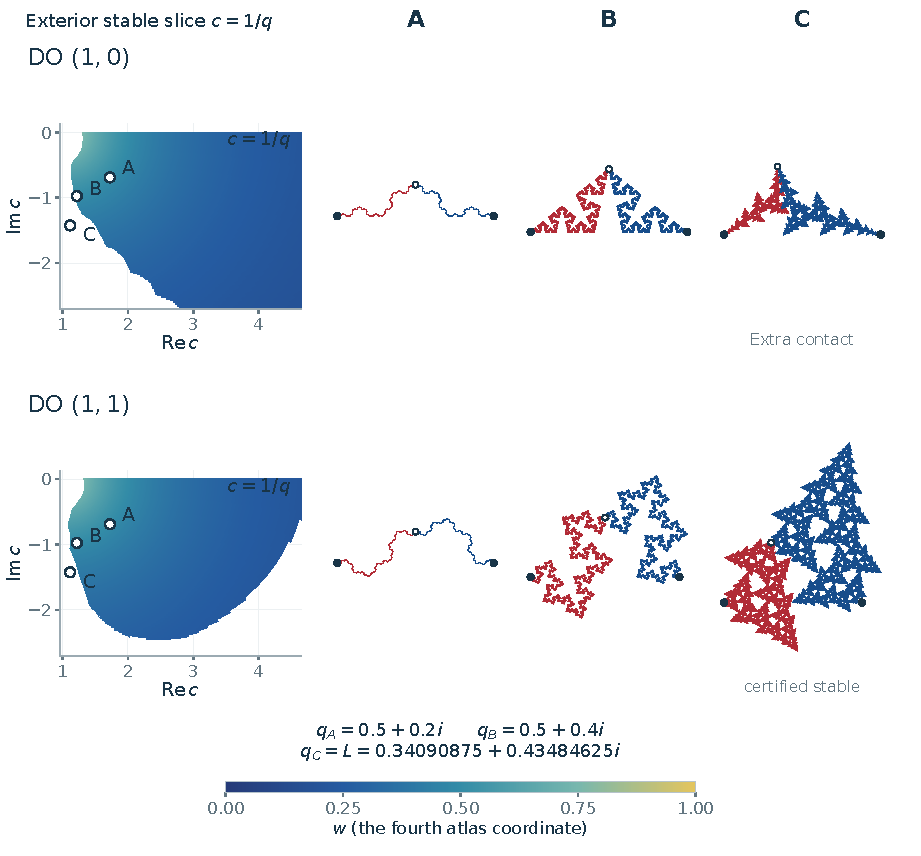
\includegraphics[width=\textwidth]{figures/four_family_DO.pdf}
\caption{DO$(1,0)$ and DO$(1,1)$ at the same exterior slice coordinates
and curve probes as Figure~\ref{fig:zipper-dd-gallery}. The opposite
map contributes the phase factor $N/\overline N$ in the canonical
exterior coefficient $c_2$. The painted slice regions certify stable
parameters. The common probe $q_C=L$ produces an additional
identification for DO$(1,0)$ and an embedded curve for DO$(1,1)$;
these conclusions come from certificates, independently of the
finite curve drawings.}
\label{fig:zipper-do-gallery}
\end{figure}

